\section{本章小结}

本章介绍了复数,重点在于复数的运算及其几何意义。复数也是一个全新的域,同样需要反复阅读概念并结合几何深入思考,同时需要和向量在乘除上的区别。

我们将向量和复数的运算的几何意义归纳如下。

\begin{table}[ht]
\centering
\begin{tabular}{ccc}
    \toprule
     & 向量 & 复数\\
    \midrule
    加减 & 平行四边形对角线 & 平行四边形对角线\\
    乘法 & 判断直角 & 旋转\\
    除法 & 无 & 旋转\\
    \bottomrule
\end{tabular}
\end{table}

根据具体形况,使用向量判断线段关系,还是使用复数计算线段夹角,需要具体问题具体分析。

~

\begin{example}[拓广探索9,难度:$\star \star \star $]
已知复数
\begin{align*}
&z_1=m+\left( 4-m^2 \right) i \qquad m\in \mathbb{R} \\
&z_2=2\cos \theta +\left( \lambda +3\sin \theta \right) i \qquad \lambda ,\theta \in \mathbb{R}
\end{align*}
并且$z_1=z_2$,求$\lambda $的取值范围。
\end{example}

解:

先考察两个复数的几何图形,均是参数方程,转化为普通方程:
\begin{align*}
&z_1:\begin{cases}
	x=m\\
	y=4-m^2\\
\end{cases}\Rightarrow \quad y=4-x^2 \\
&z_2:\begin{cases}
	x=2\cos \theta\\
	y=\lambda +3\sin \theta\\
\end{cases}\Rightarrow \quad \left( \frac{x}{2} \right) ^2+\left( \frac{y-\lambda}{3} \right) ^2=1
\end{align*}
一个开口向下的抛物线,一个椭圆。$\lambda $控制了椭圆的沿{\it y}轴的平移,要使$z_1=z_2$,即两个图形要相交,$x,y$均需有实数解。几何意义虽然明显,但全靠几何求解很难,考察代数方法,上式带入下式得到:
\[
\frac{4-y}{4}+\left( \frac{y-\lambda}{3} \right) ^2=1
\]
$y$必须在$y\leqslant 4$有实数解
\begin{align*}
&\frac{4-y}{4}+\left( \frac{y-\lambda}{3} \right) ^2=1 \\
&4y^2-\left( 8\lambda +9 \right) y+4\lambda ^2=0 \\
&\because \Delta =\left( 8\lambda +9 \right) ^2-64\lambda ^2\geqslant 0 \\
&\therefore \lambda \geqslant -\frac{9}{16}
\end{align*}
另一个可由几何获得:
\[
\lambda _{\max}=4+3=7
\]
综合得到$\lambda \in \left[ -\frac{9}{16},7 \right] $。

\begin{figure}[h]
\centering
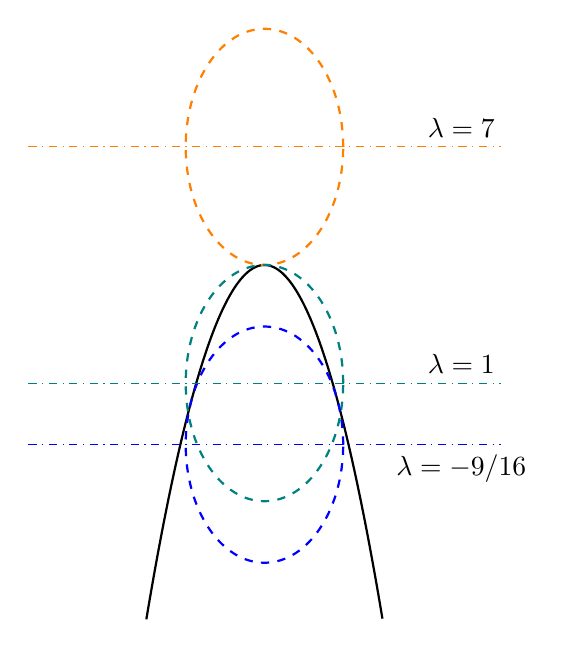
\begin{tikzpicture}[line join=round, scale=0.5]
\mydrawxy{-7}{7}{-5}{11}
\draw[thick,domain=-3:3,samples=200] plot ( \x,{4-((\x)^2)});
\draw[thick,dashed,orange] (0,7)       ellipse (2 and 3);
\draw[thick,dashed,teal]   (0,1)       ellipse (2 and 3);
\draw[thick,dashed,blue]   (0,-0.5625) ellipse (2 and 3);
\draw[dashdotted,orange] (-6,7)--(6,7);
\draw[dashdotted,teal] (-6,1)--(6,1);
\draw[dashdotted,blue] (-6,-0.5625)--(6,-0.5625);
\coordinate[label=above:{$\lambda =7$}]     (t1) at (5,7);
\coordinate[label=above:{$\lambda =1$}]     (t2) at (5,1);
\coordinate[label=below:{$\lambda =-9/16$}] (t3) at (5,-0.5625);
\end{tikzpicture}
\end{figure}

这里附带讨论交点的{\it y}坐标,如下:
\[
y=\frac{\left( 8\lambda +9 \right) \pm 3\sqrt{16\lambda +9}}{8}
\]
\begin{itemize}
    \item $\lambda <-9/16$:$y$没有实数解,两条曲线没有交点;
    \item $\lambda =-9/16$:$y_{1,2}=9/16$,两条曲线有左右2个对称的交点;
    \item $\lambda \in \left( -\frac{9}{16},1 \right) $:$y_{1,2}>0$,两条曲线有左右4个对称的交点;
    \item $\lambda =1$:$y_{1,2}=4,1/4$,两条曲线有左右2个对称的交点,和一个$\left( 0,4 \right) $,共3个交点;
    \item $\lambda \in \left( 1,7 \right) $:$y$有正有负,受$x$实数限制,取$y>0$,所以两条曲线有左右2个对称的交点;
    \item $\lambda =7$:$y_{1,2}=\frac{98}{8},4$,受$x$实数限制,取$y=4$,两条曲线只有顶部1个交点。
\end{itemize}


\begin{tcolorbox}
本题其实考察曲线的交点,结合了复数、参数方程、抛物线、椭圆。纯粹用代数非常复杂,结合几何意义就非常清晰简单。本题很有典型性,仔细研读讨论部分,XML。
\end{tcolorbox}




